\chapter{Background}
\label{sec:background}

\section{Separation Logic}

Proposed in 1969, Tony Hoare's \textit{Hoare Logic} provided a standardised
means of reasoning about programs and their correctess~\cite{hoare}. The key
principle of this logic is the Hoare Triple, denoting that if a certain
precondition $P$ holds, and code command $C$ is run (and terminates without
failing), then the postcondition $Q$ is guaranteed to hold. This is presented
in the form of a \textit{Hoare triple}, like so:

$$
  \triple{P}{C}{Q}
$$

Whilst this is a strong foundation for reasoning about programs, anything more
than the simplest of functions become hugely cumbersome to work with,
particularly concerning operations on heap-allocated memory. In 2001, Peter
O'Hearn and John Reynolds proposed \textit{Separation Logic} as the solution to
this~\cite{separation-logic}. Separation Logic reasons about
\textit{heap fragments} (sometimes called \textit{heaplets}), which represent
sections of a theoretical computer's heap; it also provides three core features
in addition to the standard Hoare Logic:

\begin{figure}
  \centering
  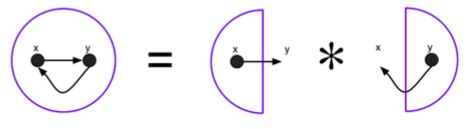
\includegraphics[width=200px]{img/separating-conjunction.jpg}
  \caption{
    A visualisation of the separating conjunction.
    From~\cite{infer-sl}.
  }
  \label{fig:separating-conjunction}
\end{figure}

\begin{itemize}
  \item The \textit{heap cell assertion}, $\cell{x}{y}$, denotes that a heap
  fragment composes of a single cell at address $x$ with value $y$.

  \item The \textit{separating conjuntion}, $P \lstar Q$, states that the heap
  fragment can be split into two disjoint (potentially empty) sub-fragments,
  one of which satisfies $P$, and the other satisfies $Q$.

  \item The \textit{Frame Rule} - a fundamental rule that allows derivations to
  temporarily ``forget'' any unneeded logic either not concerning
  heap-allocated memory, or concerning heap-allocated memory that isn't mutated
  by the command(s) currently being considered. Intuitively, this states that
  any programs that can execute on a state $P$ can also execute on a larger
  state, $P \lstar R$. The Frame Rule is as follows:

  $$
    \inferrule[Frame]{
      \triple{P}{C}{Q} \quad \mathtt{mod}(C) \cap \mathtt{fv}(R) =
      \emptyset}{\triple{P \lstar R}{C}{Q \lstar R}
    }
  $$
\end{itemize}


\section{OCaml}

Created in 1996, \textit{OCaml}~\cite{ocaml} is `an industrial-strength
programming language supporting functional, imperative and object-oriented
styles'. Specifically, OCaml provides the ability to make use of functional,
imperative, and object-oriented styles. This, combined with its powerful type
system, makes it a good fit for symbolic analysis tools. Many of Gillian's
contemporaries, including Infer~\cite{infer}, Verifast~\cite{verifast-paper,
verifast-repo}, and Frama-C~\cite{frama-c}, are also written in OCaml.

OCaml's most popular build system is \textit{Dune}~\cite{dune} - it allows the
easy compilation of multi-file OCaml programs and libraries, including
dependencies from \textit{OPAM}~\cite{opam}, OCaml's designated public library
repository. Despite Dune's popularity, it is a fairly barebones system, quickly
growing cumbersome when developing larger projects and, in particular,
switching development between projects; Dune requires that OPAM dependencies
are installed system-wide, which can lead to inconsistent builds and version
conflicts. The answer to these concerns is \textit{esy}~\cite{esy}, a package
management system for OCaml and Reason styled after \textit{npm}~\cite{npm}.
Esy provides `provides a fast and powerful workflow for local development of
opam packages without requiring ``switches''', meaning dependencies are isolated
between projects. Esy also provides a number of convenience features, such as
defining custom commands that run within the OCaml project's environment, as
well as supporting non-OPAM dependencies, e.g. OCaml sources from GitHub
repositories (optionally at a specific commit).


%% Described in Intro
%\section{Gillian}
%\section{Debugging - previous work}

\section{Related work}
\label{sec:background:related-work}

\subsection{Infer}

Facebook's \textit{Infer}~\cite{infer, infer-site} is a static analysis tool
for Java and C/C++/Objective-C, designed to use bi-abduction to provide users
with a list of potential bugs, crashes, and sources of poor performance.
Similarly to Gillian, Infer is written in OCaml, and works by compiling source
code to an intermediate representation. In contrast, Infer wholly focuses on
automated compositional testing, and refines this process to a state in which
it can easily be used in industry, whilst also including more general analysis
for concerns such as security and concurrency; it sacrifices depth of analysis
to result in a lightweight tool that gives developer-friendly feedback.

Infer doesn't require the a full program in order to perform anaylsis, as it
only needs to construct Hoare triples for one function at a time. This,
combined with its ability to reuse existing results from unchanged functions to
only consider modified code, makes for a fast and hugely scalable static
analysis tool, used as part of Facebook's code quality pipeline for all
modifications to the Android and iOS apps for Facebook, Facebook Messenger,
Instagram, and others services~\cite{infer-about}.

\subsection{VeriFast}

\textit{VeriFast}~\cite{verifast-paper, verifast-repo} `is a prototype
verification tool for single-threaded and multithreaded C and Java programs'.
VeriFast performs verification similar to Gillian, working on functions with
developer-defined pre- and post-conditions, also using an intermediate
representation to do so.

Until recent work Gillian by Matthew Ho~\cite{gillian-debugging-2021},
VeriFast's clear-cut advantage was its functioning debugger, and succinct,
immediate error reporting; as found in previous comparisons
~\cite{gillian-logging-2020}, upon attempting to verify an invalid program,
VeriFast will directly output its reasoning for the error, and the line number
responsible. While this is certainly more direct than Gillian's old method of
trawling through log files, VeriFast's error messages were often vague, and
with no produced logs to refer to for more detail, such errors often remained
cryptic.

However, VeriFast remains ahead of Gillian's debugging capabilities - whilst
Matthew's work from 2021 markedly closed the gap between the two tools (and
provided more specific and helpful error reporting, as well as some ease-of-use
features such as debugging specific functions), the DAP's limitations on
Gillian debugging left for some sorely missed features, such as the VeriFast
debugger's ability to jump to any previously executed command, and visually
show when resources allocated on the heap are freed. As of the beginning of
this project, the ability to select execution branch when debugging is absent
from both Gillian and VeriFast.

\subsection{Frama-C}

Is Frama-C worth mentioning? The only separation logic -based tooling I can
find for it is one of its older plugins, Jessie, which is no longer maintained
and currently declared potentially incompatible with more recent versions of
Frama-C.
\todo{Decide whether Frama-C is worth talking about}


\section{VSCode and its extensions}

VSCode (Visual Studio Code)~\cite{vscode} is a universally recognised text
editor and development environment, developed by Microsoft. It currently stands
as the most popular development worldwide, enjoying a 71\% market share
according to Stack Overflow's 2021 developer survey
~\cite{stack-overflow-survey-editors}.

A large factor to VSCode's success is its extensive support for extensions,
boasting over 24,000 freely-distributed extensions~\cite{vscode-popularity},
ranging from language-specific support to general developer creature comforts
(such as SSH support). Developing new extensions is made very accesible through
simple JavaScript or TypeScript projects~\cite{vscode-extensions-intro}, making
use of VSCode's well-documented API~\cite{vscode-api} to have a large degree of
control over the editor.

Whilst VSCode limits the extent to which extensions can extend the editor's UI,
extension authors are able to make use of Webviews~\cite{vscode-webview}; an
extension can open an editor tab that contains web content (HTML/CSS/JS) that
the extension has complete control over, providing a method for extensions to
fill in any gaps in VSCode's UI.

\begin{figure}
  \center
  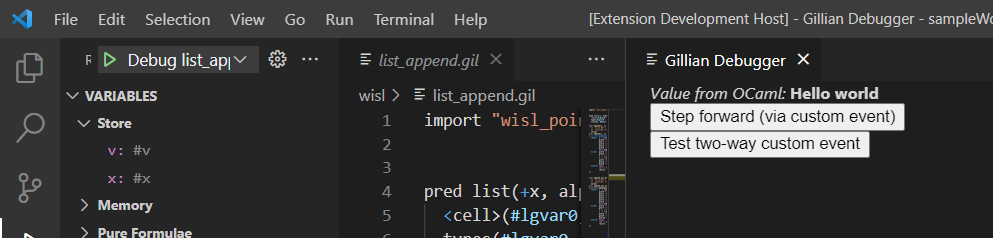
\includegraphics[width=400px]{img/webview-example.png}
  \caption{An example of a Webview created by a VSCode extension}
  \label{fig:webview-example}
\end{figure}


\begin{wrapfigure}{R}{0.5\textwidth}
  \centering
  \vspace*{-1.6cm}
  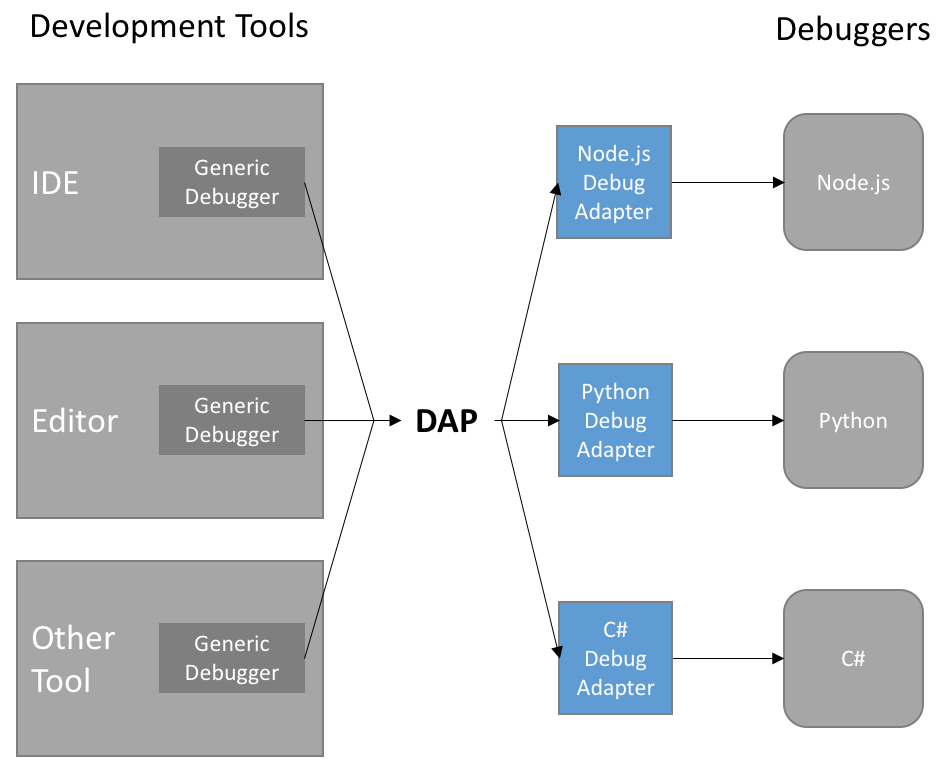
\includegraphics[width=200px]{img/dap-diagram.png}
  \vspace*{-0.45cm}
  \caption{
    The intention of the DAP, acting as an interface between arbitrary IDEs and
    arbitrary debuggers. From~\cite{dap}.
  }
  \label{fig:dap-diagram}
  \vspace*{-1cm}
\end{wrapfigure}

\subsection{Debug Adapter Protocol}
A common issue when adding IDE support for development tools is the sheer
number of editors that would ideally be supported~\cite{magpiebridge}. Whilst
VSCode has a huge market share, only supporting VSCode would neglect a
significant portion of developers. Unfortunately, maintaining support for many
editors at once is an unreasonably large undertaking. The \textit{Debug Adapter
Protocol} (DAP)~\cite{dap} exists as an attempted countermeasure to this issue,
turning the $O(m \times n)$ complexity problem of supporting many debuggers on
many editors into a $O(m + n)$ problem; each debugger and each editor need only
be integrated once.

As discussed in \autoref{sec:intro:debugging}, the DAP's limited set of
included commands proved a limiting factor in the development of a Gillian
debugger. A potential solution is to make use of custom commands and events,
which is supported both by VSCode (sending custom requests
at~\cite{vscode-dap-custom-request}, receiving custom events
at~\cite{vscode-dap-custom-event} and the OCaml DAP
implementation currently used in Gillan's debugger~\cite{ocaml-dap} (where
custom events and commands are defined similarly to those already
provided~\cite{ocaml-dap-custom}).


\subsection{Including OCaml code}

Resulting of Ocsigen's work as part of their OCaml web framework
~\cite{ocsigen-framework}, OCaml programs can be directly compiled into
JavaScript using their \texttt{Js\_of\_ocaml} package~\cite{js-of-ocaml}; by
adding a compilation flag in a project's Dune file, the relevant program can be
compiled to a \texttt{.js} file instead of a native binary. This produced file
doesn't need to be used as its own program; using the provided JS
bindings~\cite{js-of-ocaml-bindings}, the resulting JS code can export
functions and values, just like normal JS code, to be used elsewhere in a
JavaScript project.

Another option is to make use of the OCaml VSCode bindings
~\cite{vscode-ocaml-bindings} provided by OCamlLabs'
\texttt{vscode-ocaml-platform}~\cite{vscode-ocaml-platform, ocamllabs}; this
way, no JavaScript need be written at all.

These options allow the line between JavaScript and OCaml to be drawn wherever
is most opportune; the extension could be written completely in JavaScript,
requiring more attention when interacting with Gillian's debugger; the
extension could be entirely OCaml, sacrificing more succinct integration with
VSCode for a more unified codebase with Gillian; it is just as possible to draw
the line somewhere inbetween, exposing the more Gillian-related OCaml code via
functions to the JavaScript that communicates with VSCode. Additionally, both
scenarious allow for Gillian code to be shared with the extension - however,
with the Gillian libraries as they are, such libraries cannot be haphazardly
included in the extension code; \texttt{Js\_of\_ocaml} transitively includes all
OCaml dependencies, potentially leading to code that cannot be executed. As a
concrete example to this, attempting to include Gillian's \texttt{debugAdapter}
library results in erroring code, due to the compiler's attempt to include an
SQLite implimentation, which it simply is not equipped to handle. Aside from
this, the inclusion of unnecessary dependencies in JS-compiled code results in
a hugely bloated extension - the \texttt{debugAdapter} example created a
compiled JS file over a million lines long. The ideal scenario here is to move
shared Gillian code to its own library within Gillian, which has as few
dependencies as possible (ideally none), but both Gillian and the extension
code depends on.

\begin{sidewaysfigure}
  \center
  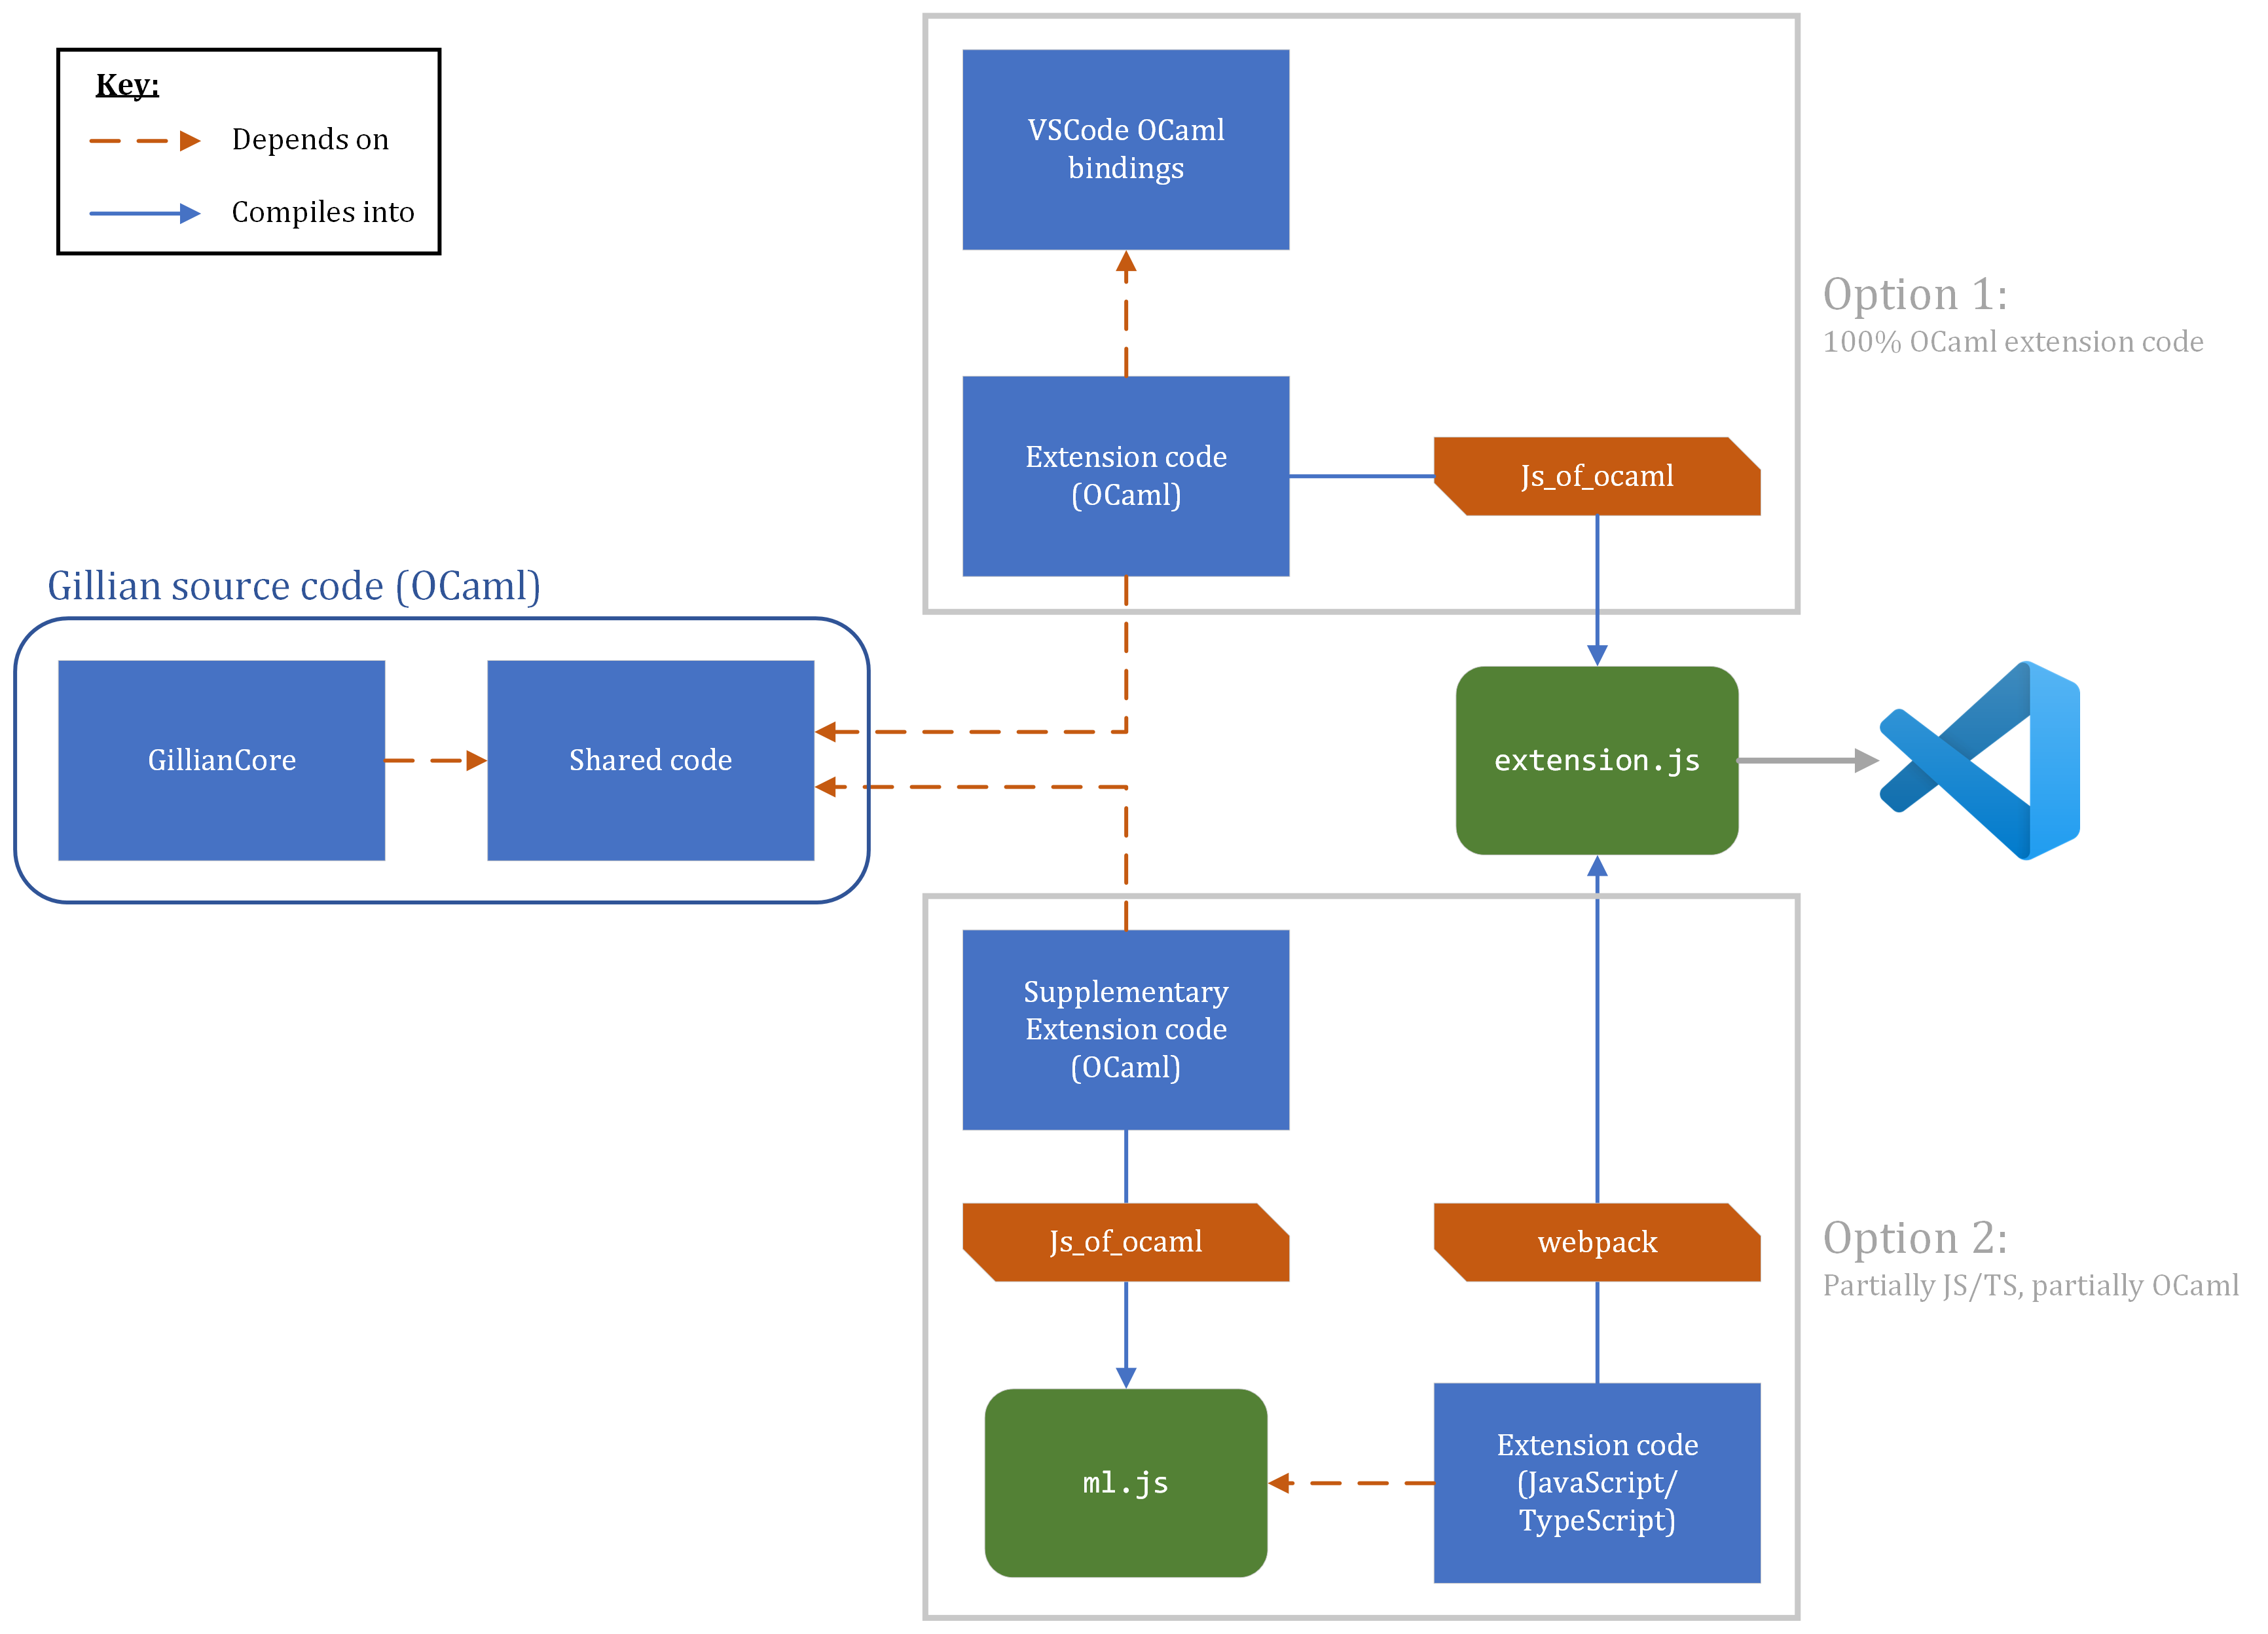
\includegraphics[width=650px]{img/vscode-extension-with-ocaml.png}
  \caption{The process of including OCaml code in a VSCode extension}
  \label{fig:vscode-extension-with-ocaml}
\end{sidewaysfigure}

\subsection{Putting it all together}
\label{sec:background:extending-dap}

A combination of DAP custom events and VSCode's Webviews can allow us to move
past DAP's initial limitations, however this comes at the cost of creating an
implementation specific to VSCode, eliminating a large benefit of using the DAP
in the first place.

A working example that tests custom DAP commands/events, Webviews and the
inclusion of OCaml code (alongside a Gillian library) is available at
\cite{debugger-experiment}.

\section{MagpieBridge}

Similar to program debugging, adding support for static code analysers to IDEs
is the amount of tools and IDEs that support must be added for. In a similar
notion to the DAP, MagpieBridge~\cite{magpiebridge} is `a framework for
integrating Static Analyses into IDEs and Editors with the Language Server
Protocol'~\cite{magpiebridge-repo}. The \textit{Language Server Protocol}
(LSP)~\cite{lsp} is another of Microsoft's creations, similar to the DAP, which
adds an arbitrary interface bridging IDEs and language tools (syntax checkers,
intellisense, etc.). As an example, MagpieBridge has provided an fully
functional integration for Infer~\cite{infer-ide}.

A particular feature of MagpieBridge is its ability to serve a configuration
webpage, in which the user can configure the static analysis in their browser
of choice. Unfortunately, this pre-generated page can't contain any custom
content, and can only be used for configuration - this would prohibit advanced
debugging features from being served driectly from a MagpieBridge server.

Additionally, the inclusion of MagpieBridge would involve the addition of Java
to the language base of Gillian, increasing complexity of the project and
potentially harming long-term usability.


\begin{figure}
  \noindent
  \makebox[\textwidth]{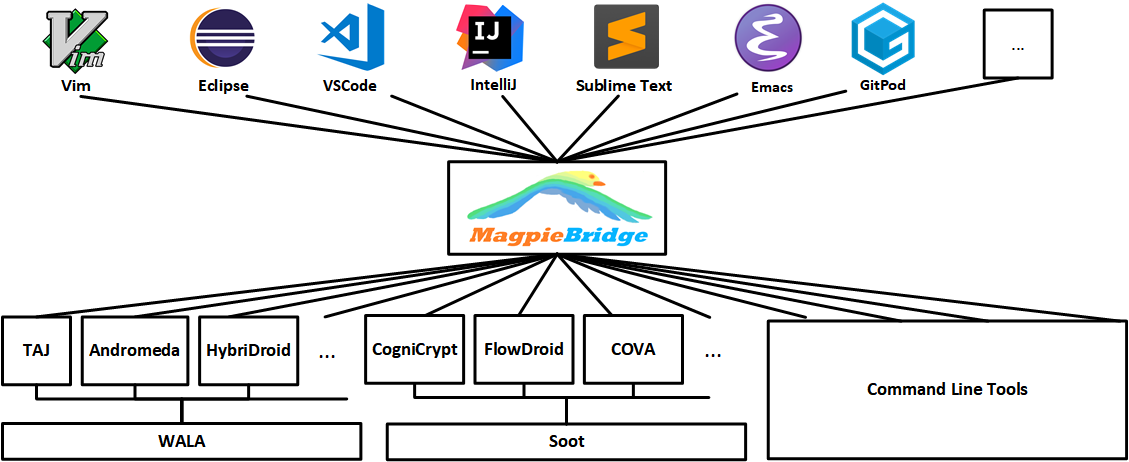
\includegraphics[width=500px]{img/magpiebridge-goal.png}}
  \caption{
    The goal of MagpieBridge; bridging static analysis tools with IDEs.
    From~\cite{magpiebridge-repo}.
  }
  \label{fig:webview-example}
\end{figure}
